
%\section{Module 4: Refrigeration and Liquefaction}

%%%
%\section{Gas Refrigeration Cycles}

\begin{center}
\begin{tabular}{||c||}
\hline \hline
Thermodynamic Tables for the fluids used in this  \\
list can be found in any Textbook or be downloaded from \\
  \\
\href{https://highered.mcgraw-hill.com/sites/dl/free/0073529214/395307/appdxs1_2.pdf}{https://highered.mcgraw-hill.com/sites/dl/free/0073529214/395307/appdxs1$\_$2.pdf} \\
\hline\hline
\end{tabular}
\end{center}

\begin{enumerate}
%%%
%%% Saphiro 10.53 (7th Ed.)
%%% 
\item \label{Ex1} {\it In a Brayton refrigeration cycle with regenerative heat exchanger, air enters the compressor at -6.15$^{\text{o}}$C and 1.0 bar, and is compressed isentropically to 2.70 bar. The compressed air enters the regenerative heat exchanger at 26.85$^{\text{o}}$C and is cooled to -6.15$^{\text{o}}$C before entering the turbine where is expanded isentropically (Fig. \ref{Ex1:Fig}). If the refrigeration capacity is 15 tons, calculate:
\begin{enumerate}
\item volumetric flow rate at the compressor inlet $\left(\text{m}^{3}/\text{min}\right)$;
\item coefficient of performance.
\end{enumerate}
}


\begin{figure}[h]
\begin{center}
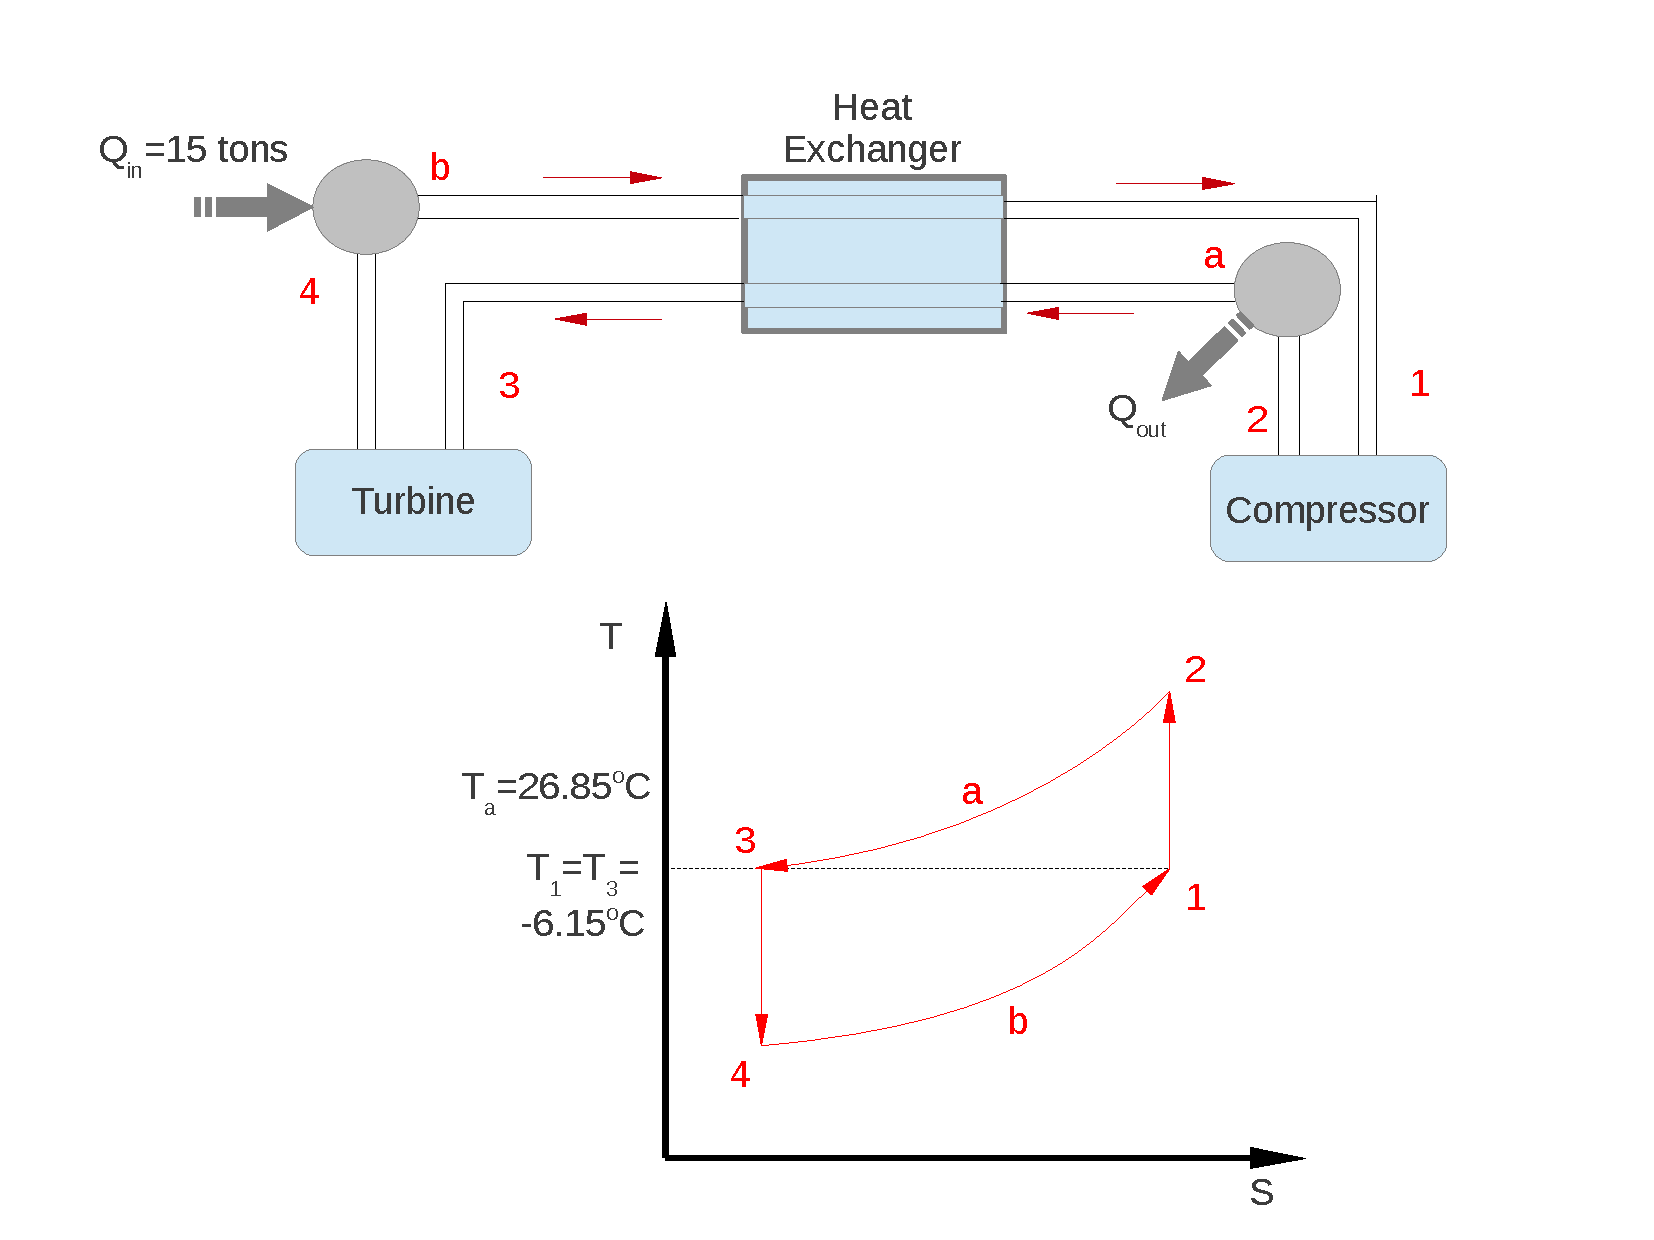
\includegraphics[width=13.0cm,height=10.0cm]{./Pics/Overview_Refrig11}
\end{center}
\caption{Gas refrigeration cycle: Problem \ref{Ex1}.}\label{Ex1:Fig}
\end{figure}

Let's first assume that there is no heat transfer from the heat exchanger to its surroundings. For each state shown in Fig. \ref{Ex1:Fig} we can extract the relevant data from the ideal gas properties of air tables\footnote{Moran, Shapiro, Boettner and Bailey; $\lq$Principles of Engineering Thermodynamics', Table A-22 (Seventh Edition).} 
\begin{itemize}
\item {\bf State 1:} At $T_{1}=-6.15^{\text{o}}\text{C}=267\text{ K}$ and $P_{1}=1$ bar\\
\begin{tabular}{ c c c }
{\bf T (K)} & {\bf H (kJ/kg)}  & {\bf P$_{r}$} \\
  260       &   260.09         &    0.8405  \\
  270       &   270.11         &    0.9590  \\
\end{tabular}

From linear interpolation $H_{1}$=267.10 kJ/kg and P$_{r,1}$=0.9235\footnote{Starting from the entropy definition, as a function of enthalpy and pressure, 
\begin{displaymath}
TdS=dH-VdP \rightarrow dS=\frc{dH}{T}-\frc{V}{T}dP
\end{displaymath}
Integrating the expression above from state 1 to state 2 and for ideal gas, $\frc{V}{T}=\frc{R}{P}$:
\begin{equation}
S\left(T_{2},P_{2}\right) - S\left(T_{1},P_{1}\right)=\int\limits_{T_{1}}^{T_{2}}C_{p}(T)\frc{dT}{T}-R\ln\frc{P_{2}}{P_{1}}\label{EqnEntropy}
\end{equation}
For an arbitrary reference temperature $\left(T_{r}\right)$ the second integral in the rhs can be rewritten as the integral difference:
\begin{displaymath}
\int\limits_{T_{1}}^{T_{2}}C_{p}\frc{dT}{T}=\int\limits_{T_{r}}^{T_{2}}C_{p}\frc{dT}{T} - \int\limits_{T_{r}}^{T_{1}}C_{p}\frc{dT}{T} = S^{\text{o}}\left(T_{2}\right)-S^{\text{o}}\left(T_{1}\right)
\end{displaymath}
where $S^{\text{o}}\left(T_{2}\right)$ and $S^{\text{o}}\left(T_{1}\right)$ depend {\bf only} on the temperature and can be easily tabulated in the same way as it is done for $H$ and $U$.  Thus for isentropic processes, Eqn. \ref{EqnEntropy} becomes
\begin{displaymath}
0 = S^{\text{o}}\left(T_{2}\right)-S^{\text{o}}\left(T_{1}\right) - R\ln\frc{P_{2}}{P_{1}}
\end{displaymath}
This equation can be easily manipulated,
\begin{displaymath}
\textcolor{red}{\frc{P_{2}}{P_{1}}} = \frc{\exp\left[S^{\text{o}}\left(T_{2}\right)/R\right]} {\exp\left[S^{\text{o}}\left(T_{1}\right)/R\right]} = \textcolor{red}{\frc{P_{r,2}}{P_{r,1}}}
\end{displaymath}
$P_{r}=P_{r}(T)$ is called {\it relative pressure}.}

\item {\bf State 2:} $P_{2}=2.80$ bar and as \textcolor{red}{1-2} is isentropic, we can use the {\it relative pressure} to calculate $H_{2}$,
\begin{displaymath}
\frc{P_{r,2}}{P_{r,1}} = \frc{P_{2}}{P_{1}} \Longrightarrow P_{r,2} = P_{r,1}\frc{P_{2}}{P_{1}} = 2.4935
\end{displaymath}
From the  ideal gas properties of air table,\\
\begin{tabular}{ c c c }
{\bf T (K)} & {\bf H (kJ/kg)}  & {\bf P$_{r}$} \\
  350       &   350.49         &    2.379  \\
  360       &   360.58         &    2.626  \\
\end{tabular}

$H_{2}=355.17$ kJ/kg, $T_{2}=354.63$ K$ = 81.48 ^{\text{o}}$C

\item {\bf State a:} $T_{a}=26.85^{\text{o}}$C$=300$ K $\Longrightarrow$ $H_{a}=300.19$ kJ/kg.

\item {\bf State 3:} $T_{3}=T_{1}=-6.15^{\text{o}}\text{C}=267\text{ K} \Longrightarrow$ $H_{3}$=267.10 kJ/kg and P$_{r,3}$=0.9235

\item {\bf State 4:} Similarly to state 2 and remembering that in Brayton cycles $P_{2}=P_{3}$ and $P_{1}=P_{4}$: 
\begin{displaymath}
P_{r,4} = P_{r,3}\frc{P_{4}}{P_{3}} = P_{r,3}\frc{P_{1}}{P_{2}} = 0.3420
\end{displaymath}
and from the ideal gas properties of air table, \\
\begin{tabular}{ c c c }
{\bf T (K)} & {\bf H (kJ/kg)}  & {\bf P$_{r}$} \\
  200       &   199.97         &    0.3363  \\
  210       &   209.97         &    0.3987 \\
\end{tabular}

From linear interpolation $H_{4}=200.88$ kJ/kg and $T_{4}=200.91$ K $= -72.24^{\text{o}}$C.

\item {\bf State b:} A simple energy balance in the heat exchanger (assuming that no heat is lost/gained to/from the surroundings)
\begin{displaymath}
\left(H_{b}-H_{1}\right) + \left(H_{a}-H_{3}\right) = 0 \Rightarrow H_{b} = -(300.19-267.10)+267.10 = 234.01 \text{ kJ/kg}
\end{displaymath}
\end{itemize}

With the given refrigeration capacity, the air mass flow rate is
\begin{displaymath}
\dot{m} = \frc{\dot{Q}_{in}}{\left(H_{b}-H_{4}\right)} = \frc{15 [tons]}{234.01-200.88 [kJ/kg]}\times \frc{1.4\times 10^{4}\;\;[kJ/h]}{1\;\;[ton]}=6338.67 \text{ kg/h}
\end{displaymath}
And the volumetric flow rate at the compressor intake is (molecular weight of dry air is 28.97 g/gmol):
\begin{eqnarray}
\textcolor{red}{\dot{V}} &=& \frc{\dot{m}RT_{1}}{P_{1}} = \frc{6338.67\left[\frc{kg}{h}\right] \times 8.314\times 10^{-5}\left[\frc{m^{3}.bar}{gmol.K}\right]\times 267\;[K]\times \left[\frc{1\;gmol}{28.97\;g}\right]\times \left[\frc{1000\;g}{1\;kg}\right]\times\frc{1\;[h]}{60\;[min]}}{1\;[bar]} \nonumber \\
&=& \textcolor{red}{80.95 \frc{\text{m}^{3}}{\text{min}}} \nonumber
\end{eqnarray}

The coefficient of performance (COP) is
\begin{displaymath}
\textcolor{red}{\text{COP}} = \frc{\text{Refrigerant Effect}}{\text{Work done}} = \frc{H_{b}-H_{4}}{\left(H_{2}-H_{1}\right)-\left(H_{3}-H_{4}\right)} = \frc{234.01 - 200.88}{(355.17-267.10)-(267.10-200.88)} = \textcolor{red}{1.516}
\end{displaymath}

%%%
%%% Saphiro 10.54 (7th Ed.)
%%% 
\item \label{Ex2} {\it Assume now that the compressor and turbine of  Problem \ref{Ex1} have isentropic efficiencies of 88$\%$. Answer the same questions for the modified cycle as in Problem \ref{Ex1}.}


%%%
%%% Saphiro 10.57 (7th Ed.)
%%% 
\item \label{Ex3}{\it  Air undergoes a Stirling refrigeration cycle. At the beginning of the isothermal compression, the pressure and temperature are 100 kPa and 300 K, respectively. The compression ratio is 6, and the temperature during the isothermal expansion is 100 K. Calculate:
\begin{enumerate}
\item The heat transfer during the isothermal expansion in kJ/kg of air;
\item The net work for the cycle in kJ/kg of air;
\item The coefficient of performance.
\end{enumerate}  
}

\begin{figure}[h]
 \begin{center}
  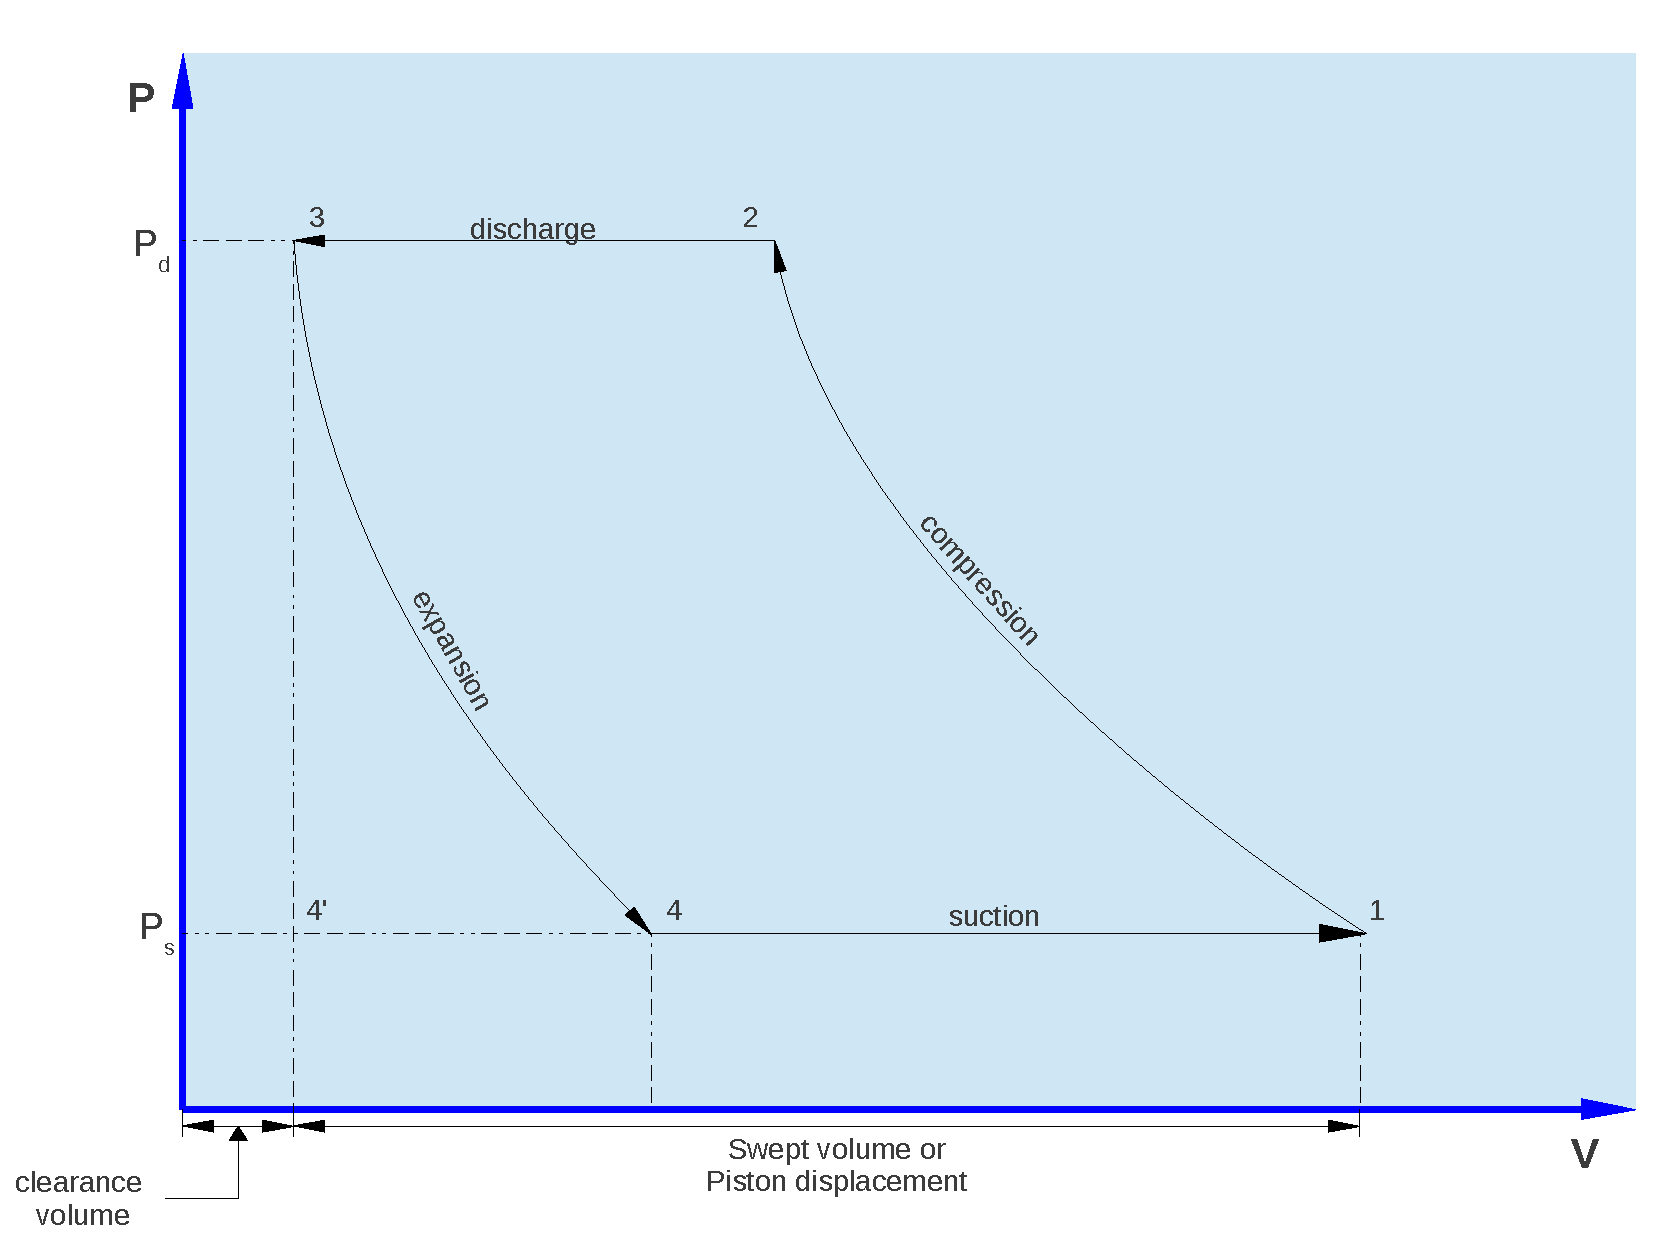
\includegraphics[width=12.cm,height=8.cm,clip]{./Pics/Overview_Refrig29}
  \end{center}
  \caption{Strokes in the compressor: Problem \ref{Ex4}.}\label{ex4_pic}
\end{figure}  


%%%
%%% Rajput (pg 739-40)
%%%
\item \label{Ex4} {\it Derive the clearance volumetric efficiency $\left(\eta_{cv}\right)$ expression in a compressor (Fig. \ref{ex4_pic}) assuming polytropic expansion.}
During the compression stage (Fig. \ref{ex4_pic}) in the refrigeration cycle, the motion of the piston within the cylinder can be described by the four strokes:
\begin{itemize}
\item (4-1): suction;
\item (1-2): compression;
\item (2-3): discharge;
\item (3-4): expansion;
\item (4-1): suction.
\end{itemize}
During the suction stroke (4-1), the vapour contained in the clearance space of the cylinder at the discharge pressure, $P_{d}$, expands (3-4). The suction valve is opened when the pressure drops to the suction pressure -- $P_{s}$, and the volume sucked is $\left(V_{1}-V_{4}\right)$ whereas the swept volume is $\left(V_{1}-V_{4}'\right)$.  The clearance volumetric efficiency is formally defined as,
\begin{equation}
\eta_{cv}=\frc{V_{1}-V_{4}}{V_{1}-V_{4'}}=\frc{V_{1}-V_{4}}{V_{1}-V_{3}} 
\label{clearancevolumetricefficiency}
\end{equation}
In a polytropic expansion process (3-4),
\begin{eqnarray}
 P_{3}V_{3}^{n} = P_{4}V_{4}^{n} &\Longrightarrow& P_{d}V_{3}^{n}=P_{s}V_{4}^{n} \nonumber \\
&& V_{4}=V_{3}\left(\frc{P_{d}}{P_{s}}\right)^{1/n} \label{polytropic}
\end{eqnarray}
We define the clearance ratio as
\begin{displaymath}
\mathcal{C}=\frc{\text{Clearance Volume}}{\text{Swept Volume}} = \frc{V_{3}}{V_{1}-V_{3}}
\end{displaymath}

Rearranging Eqn. \ref{clearancevolumetricefficiency},
\begin{eqnarray}
\eta_{cv} &=& \frc{V_{1}-V_{4}}{V_{1}-V_{3}} = \frc{\left(V_{1}-V_{4'}\right)-\left(V_{4}-V_{4'}\right)}{V_{1}-V_{3}} = \frc{\left(V_{1}-V_{3}\right)-\left(V_{4}-V_{3}\right)}{V_{1}-V_{3}} \nonumber \\
         &=& 1 - \frc{V_{4}-V_{3}}{V_{1}-V_{3}} \nonumber
\end{eqnarray}
Now substituting $V_{4}$ from Eqn. \ref{polytropic},
\begin{eqnarray}
\textcolor{blue}{\eta_{cv}} &=& 1 - \frc{V_{3}\left(\frc{P_{d}}{P_{s}}\right)^{1/n}-V_{3}}{V_{1}-V_{3}}=1+\frc{V_{3}}{V_{1}-V_{3}}\left[1-\left(\frc{P_{d}}{P_{s}}\right)^{1/n}\right] \nonumber \\
         &=& \textcolor{blue}{1 + \mathcal{C}\left[1-\left(\frc{P_{d}}{P_{s}}\right)^{1/n}\right]}
\end{eqnarray}

%%%
%%% Ameen (example 3.3, pg 50)
%%%
\item \label{Ex5} {\it An ice plant operates on the ideal vapour-compression cycle with superheated state using refrigerant fluid R134a.  The refrigerant enters the compressor as saturated vapour at 0.15 MPa and leaves the condenser as saturated liquid at 0.7 MPa.  Water enters the refrigerator cavity at 30$^{\text{o}}$C and leaves as ice at -5$^{\text{o}}$C. For an ice production rate of 10 kg per hour, determine the power input to the ice plant and the COP of the cycle. Also, sketch the $PH$ and $TS$ diagrams. Specific heats of ice and water are 2.1 and 4.18 kJ/(kg.K), respectively, and the latent heat of fusion of ice is 334 kJ/kg. Repeat the same procedure for ammonia and propane as refrigerat fluid.}


%%%
%%% Ameen (example 3.9, pg 60)
%%%
\item \label{Ex6} {\it In an ammonia refrigeration system, the evaporator supplies 300kW of refrigeration at -30$^{\text{o}}$C.  The system uses 2-stage compression as shown in the Fig. \ref{fig:ex6}, with intercooling and removal of flash gas.  The condensing temperature is 35$^{\text{o}}$C.
    \begin{enumerate}
     \item Sketch the $PH$ diagram;
     \item Calculate the power required by the compressors;
     \item Determine the coefficient of performance.
    \end{enumerate}

Assume that the intermediate pressure is expressed as: $P_{i}=\sqrt{P_{5}P_{1}}$.}
   \begin{figure}[h]
    \begin{center}
     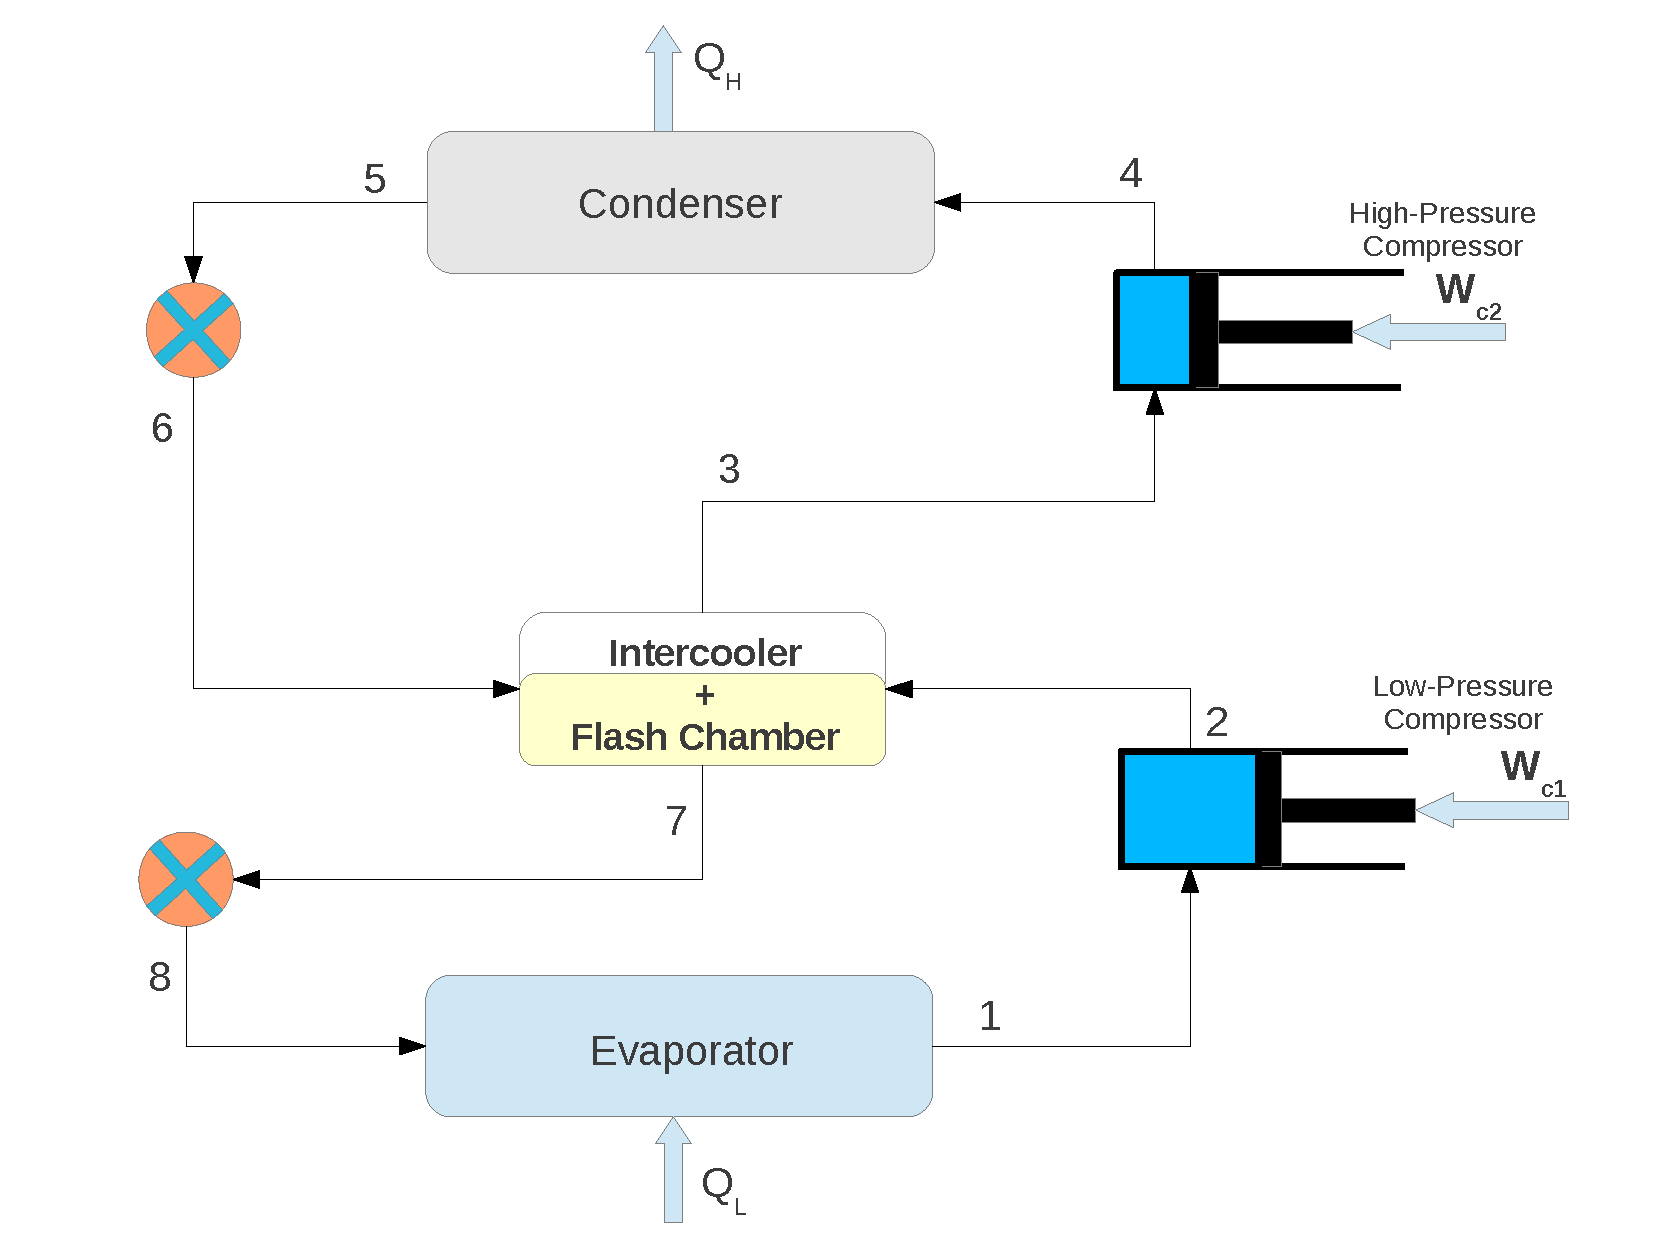
\includegraphics[width=10.cm,height=10.cm,clip]{./Pics/Overview_Refrig30}
    \end{center}
     \caption{Two-stage vapour-compression cycle: Problems \ref{Ex6} and \ref{Ex9}.} \label{fig:ex6} 
  \end{figure}  


%%%
%%% Saphiro 10.15
%%%
\item \label{Ex7} {\it A vapour-compression refrigeration cycle operates with Refrigerant R-134a as refrigerant fluid. Saturated vapour enters the compressor at 2 bar, and saturated liquid exits the condenser at 8 bar. The isentropic compressor efficiency is of 80$\%$. The mass flow rate  of refrigerant is 7 kg/min. Determine:
\begin{enumerate}
\item Compressor power;
\item Refrigerant effect (in tons and in kJ/s) and;
\item COP.
\end{enumerate}
}

%%%
%%% Saphiro 10.21
%%%
\item \label{Ex8} {\it In a vapour-compression refrigeration cycle operating with ammonia as refrigerant fluid, the refrigerating capacity is of 150 kW. Ammonia leaves the evaporator as saturated vapor at -22$^{\text{o}}$C and is driven to the condenser at 16 bar and 160$^{\text{o}}$C and leaves as saturated liquid at 16 bar. Assume that there is no relevant mechanical or thermal energy losses in and between the components of the cycle and also with the surroundings. Determine:
\begin{enumerate}
\item Mass flow rate of the refrigerant in kg/s;
\item Power input to the compressor in kW;
\item COP;
\item isentropic efficiency of the compressor.
\end{enumerate} 
}


%%%
%%% Saphiro 10.30
%%%
\item \label{Ex9} {\it An ammonia-based two-stage vapour-compression refrigeration system (Fig. \ref{fig:ex6}) uses a direct contact heat exchanger to achieve inter-cooling. The evaporator has a refrigerating capacity of 30 tons and produces -30$^{\text{o}}$C saturated vapour at its exit. In the first compressor stage, ammonia is compressed adiabatically to 5.5 bar, which is the pressure in the direct contact heat exchanger. Saturated vapour at 5.5 bar enters the second compressor stage and is compressed adiabatically to 18 bar.  Each compressor stage has an isentropic efficiency of 85$\%$. Assume that there are no mechanical or thermal energy losses within the cycle and to the surroundings. Saturated liquid enters each expansion valve. Determine:
\begin{enumerate}
\item The ratio of mass flow rates $\dot{m}_{3}/\dot{m}_{1}$;
\item Power input to each compressor stage $\left(W_{c,1},\;W_{c,2}\right)$;
\item COP.
\end{enumerate}
}


%%%
%%% Rajput Ex 14.24
%%%
\item \label{Ex10} {\it A heat pump operates in a vapour-compression cycle using Refrigerant-22 (R-22) as working fluid.  R-22 is compressed from saturated vapour at 2 bar to the condenser pressure of 12 bar.  The isentropic efficiency of the compressor is of 80$\%$. Saturated liquid enters the throttling valve at 12 bar. 80$\%$ of the heat rejected is transferred to the heated space which has a total heating requirement of 500 kJ/min. Determine:
\begin{enumerate}
\item (A)-(H) in the Table below:

%\begin{table}[h]
\begin{center}
\begin{tabular}{ || c || c | c | c | c || }
\hline\hline
        & {\bf Pressure}  &  {\bf Enthalpy}  & {\bf Entropy}     & {\bf State}  \\
        & {\bf (bar)}     &  {\bf (kJ/kg)}   &  {\bf (kJ/kg.K)}  &              \\
\hline\hline
{\bf 1} &   2.0           &       (A)        &      (B)          &  Saturated Vapour \\
{\bf 2} &   12.0          &       (C)        &      --           &  (D)          \\
{\bf 3} &   12.0          &       (E)        &      --           &  (F)        \\
{\bf 4} &   --            &       (G)        &      --           &  (H)       \\ 
\hline\hline
\end{tabular}
\end{center}
%\end{table}

\item Mass flow rate of the R-22 in kg/min.
\item Actual work in the compressor.
\item Coefficient of performance.

\end{enumerate}

}


%%%
%%% Rajput 14.19 modified
%%%
\item \label{Ex11} {\it A refrigerant fluid in a single-stage vapour-compression cycle produces a refrigerant capacity of 35 kW (thermodynamics properties in the table below). Saturated vapour leaves the evaporator at 1.50 bar and is compressed into superheated vapour at 9.0 bar. Determine
\begin{enumerate}
\item Mass flow rate of the refrigerant;
\item Power given to the compressor;
\item Piston displacement assuming that the expansion stroke follows $PV^{1.21}$ = constant. The volumetric efficiency of the piston is given by
\begin{displaymath}
\eta_{vol}=1 + \mathcal{C} - \mathcal{C} \left(\frac{P_{d}}{P_{s}}\right)^{n}
\end{displaymath}
where $\mathcal{C}$ is the clearance ratio, $P_{d}$ and $P_{s}$ are the discharge and suction pressures, respectively. The compressor operates at 150 rpm and has a clearance volume of 1.5$\%$ of the stroke volume.
\item Sketch the $TS$ diagram of the refrigeration process and the $PV$ diagram of the strokes in the compressor.
\end{enumerate}
Assume that the heat capacity of the fluid is $C_{p}=4.818$ kJ/(kg.K).
\begin{center}
\begin{tabular}{|c c| c c c c c | }
\hline
$P$             & $T_{s}$  & $V_{g}$  & $H_{f}$  & $H_{g}$   &  $S_{f}$   &  $S_{g}$    \\
(bar)   &  ($^{\text{o}}$C)  & $\left(\text{m}^{3}/\text{kg}\right)$ & (kJ/kg) & (kJ/kg) & (kJ/(kg.K)) &  (kJ/(kg.K))  \\
\hline
1.50  &  -25.22  & 0.7787 & 65.32 & 1410.61 & 0.2712 & 5.6973  \\
9.00  &   21.52  & --     & 281.53 & 1460.97 & 1.0649 & 5.0675  \\
\hline
\end{tabular}
\end{center}
}

%%%
%%% Shapiro 10.31
%%%
\item \label{Ex12} {\it Ammonia is used as a refrigerant fluid in a 2-stage vapour-compression refrigeration system (Fig. \ref{Ex12:Fig}) with 2 evaporators and a heat exchanger. Saturated vapour from the evaporator 1 enters the compressor 1 at 1.2 bar and exits at 5 bar. Evaporator 2 operates at 5 bar with saturated vapour exiting towards the heat exchanger. The condenser pressure is 14 bar and saturated liquid exits the condenser. Each compressor stage has an isentropic efficiency of 80$\%$. The refrigeration capacity of evaporators 1 and 2 are of 5 and 10 tons, respectively. 
\begin{enumerate}
 \item Determine the temperature of the ammonia at the exit of each evaporator.
 \item Calculate the power input to each compressor and the overall coefficient of performance of the cycle.
 \item Sketch the TS diagram of the cycle.
\end{enumerate}

}

\begin{figure}[h]
\begin{center}
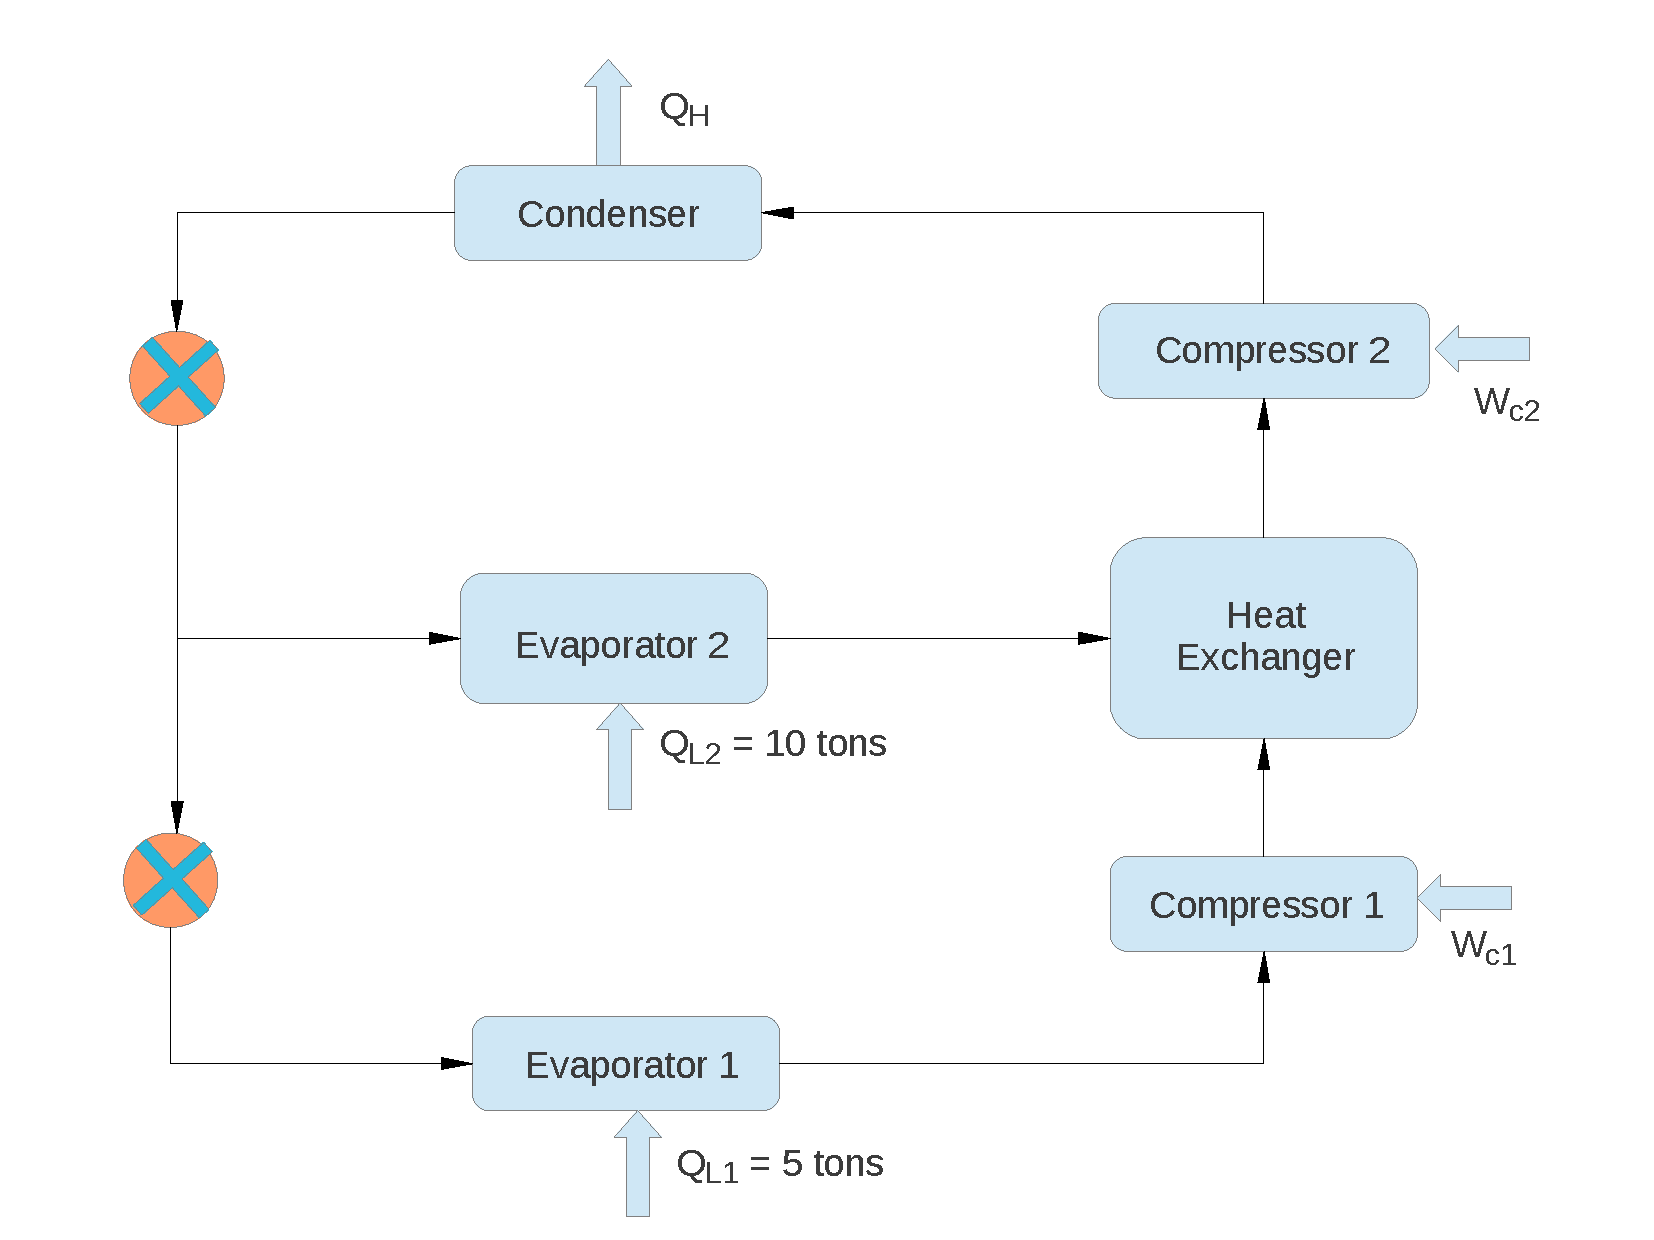
\includegraphics[width=16.0cm,height=12.0cm]{./Pics/Overview_Refrig41}
\end{center}
\caption{Two-stage vapour-compression refrigeration cycle: Problem \ref{Ex12}.}\label{Ex12:Fig}
\end{figure}




%%%
%%% Shapiro 10.42
%%%
\item \label{Ex13} {\it R-22 is the refrigerant fluid in a geothermal heat pump system for a house (Fig. \ref{Ex13:Fig}). The heat pump uses underground water from a well $\left(T_{\text{w}}^{\text{in}}=13^{\text{o}}\text{C}; T_{\text{w}}^{\text{out}}=7^{\text{o}}\text{C}\right)$ to produce a heating capacity of 4.2 tons. Determine:
\begin{enumerate}
 \item Volumetric flow rate of heated air to the house $\left(m^{3}/s\right)$;
 \item Isentropic efficiency $\left(\eta_{c}\right)$ and power $\left(\dot{W}_{c}\right)$ of the compressor;
 \item Coefficient of Performance;
 \item Volumetric flow rate of water from the geothermal well $\left(l/h\right)$;
 \item Sketch the $TS$ diagram.
\end{enumerate}
Given the heat capacity $\left(C_{p}^{\text{air}}=1.004\displaystyle\frac{kJ}{kg.K}\right)$ and molecular weight $\left(MW^{\text{air}}=28.97\displaystyle\frac{kg}{kgmol}\right)$ of air and heat capacity of water $\left(C_{p}^{\text{water}}=4.1813\displaystyle\frac{kJ}{kg.K}\right)$.
}

\begin{figure}[h]
\begin{center}
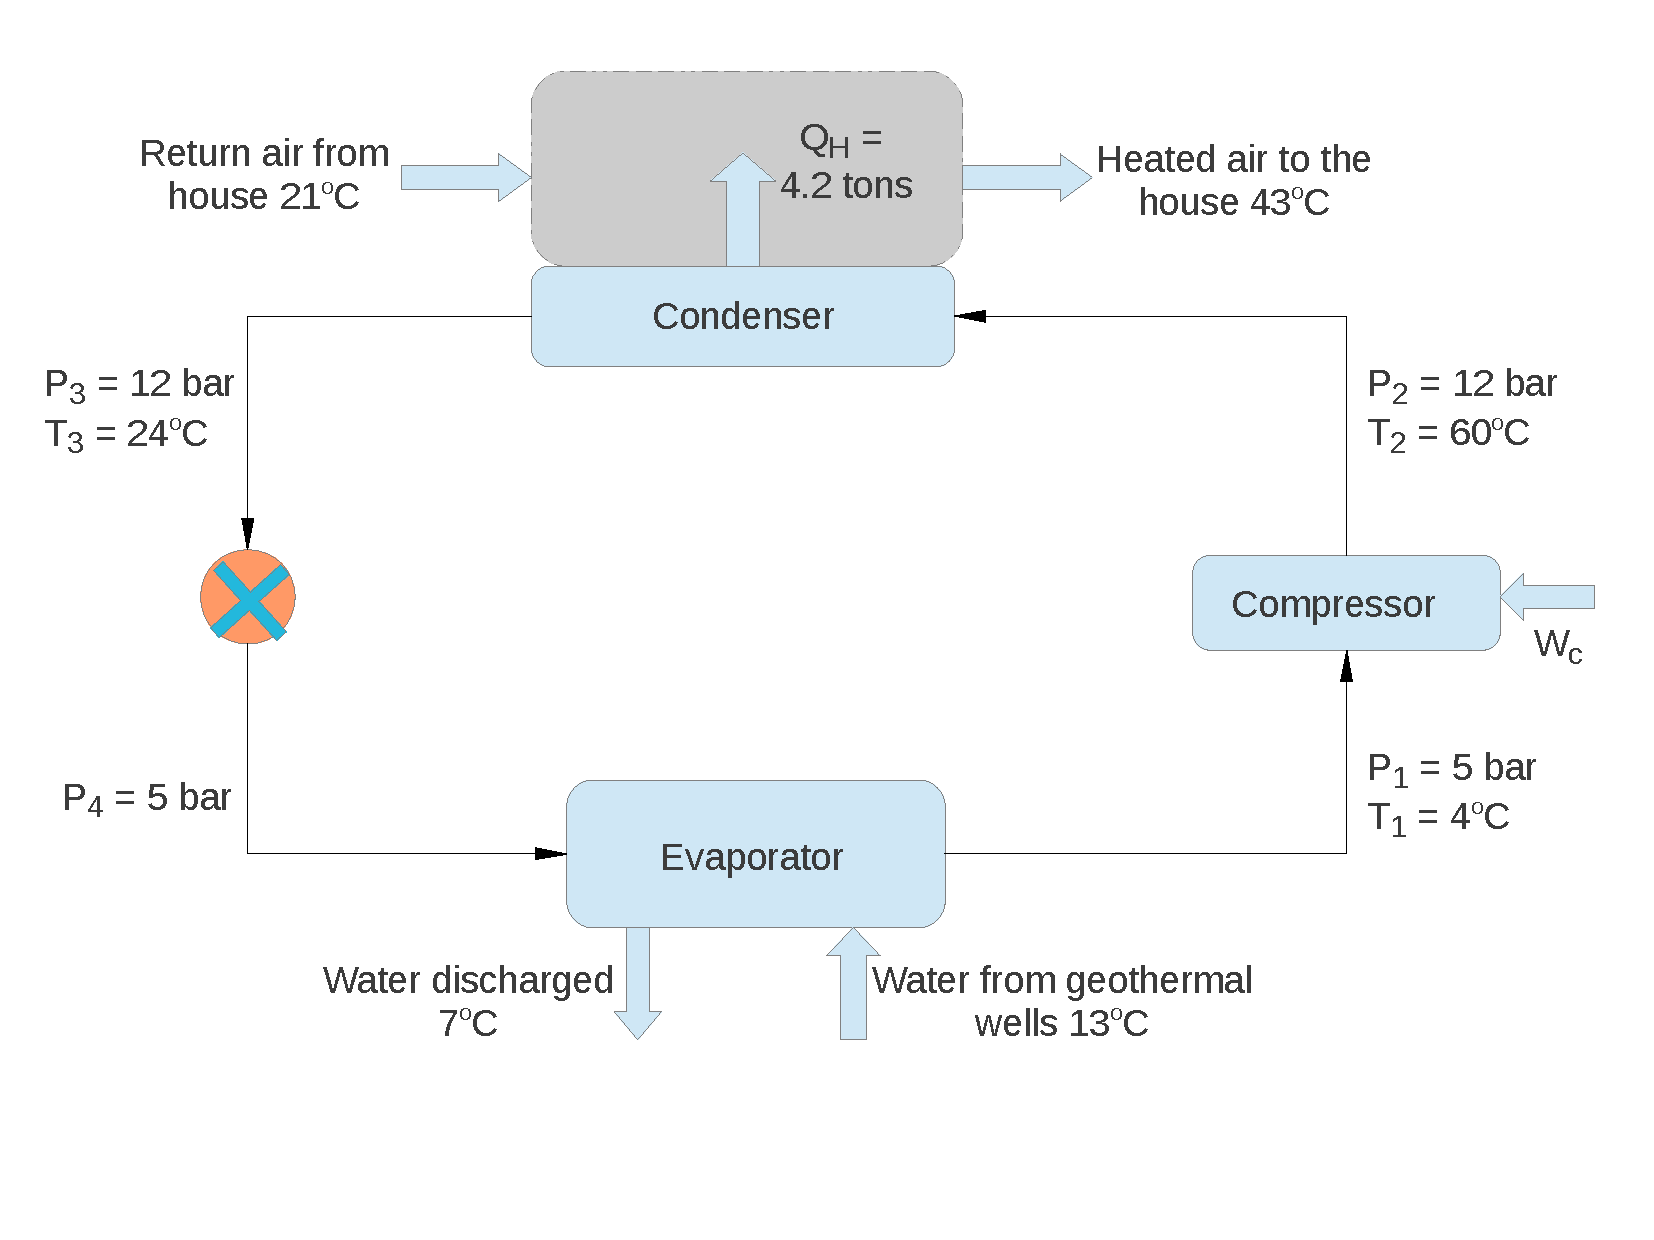
\includegraphics[width=16.0cm,height=12.0cm]{./Pics/Overview_Refrig42}
\end{center}
\caption{Heat pump cycle: Problem \ref{Ex13}.}\label{Ex13:Fig}
\end{figure}


\pagebreak

%%%
%%% Jeff
%%%
\item \label{Ex14} {\it A Thermal engineer is hired to design coupled steam-power and refrigeration plants (Fig. \ref{Ex14:Fig}). The thermal plant (I) operates 100 kg/h steam in 3-turbines reheat Rankine cycle with initial conditions and efficiencies described in Tables \ref{Ex14:Tab1} and \ref{Ex14:Tab2}. 0.1$\%$ of the power generated by the set of turbines in {\bf I} is used in the compressor of the refrigeration unit {\bf II}. The refrigeration system operates with a proprietary working fluid, $\mathcal{X}$ with thermodynamic properties as described in Table \ref{Ex14:Tab3}. Determine:
\begin{enumerate}
\item Net work for the thermal cycle {\bf I} $\left(\displaystyle\frac{\dot{W}_{\text{cycle}}}{\dot{m}_{\text{water}}}\right)$ and the power produced by the set of turbines $\left(\dot{W}_{c}\right)$;
\item Extensive properties of units {\bf I} and {\bf II} in Table \ref{Ex14:Tab1} -- {\bf A}-{\bf V} and {\bf i}-{\bf xii};
\item Mass flow rate of refrigerant fluid $\mathcal{X}$ and refrigerating capacity;
\item Piston displacement assuming that the expansion stroke follows $PV^{1.3}$ = constant. The volumetric efficiency of the piston is given by
\begin{displaymath}
\eta_{vol}=1 + \mathcal{C} - \mathcal{C} \left(\frac{P_{d}}{P_{s}}\right)^{n}
\end{displaymath}
where $\mathcal{C}$ is the clearance ratio, $P_{d}$ and $P_{s}$ are the discharge and suction pressures, respectively. The compressor operates at 360 rpm and has a clearance volume of 4$\%$ of the stroke volume.
\end{enumerate}

}

\begin{figure}[h]
\begin{center}
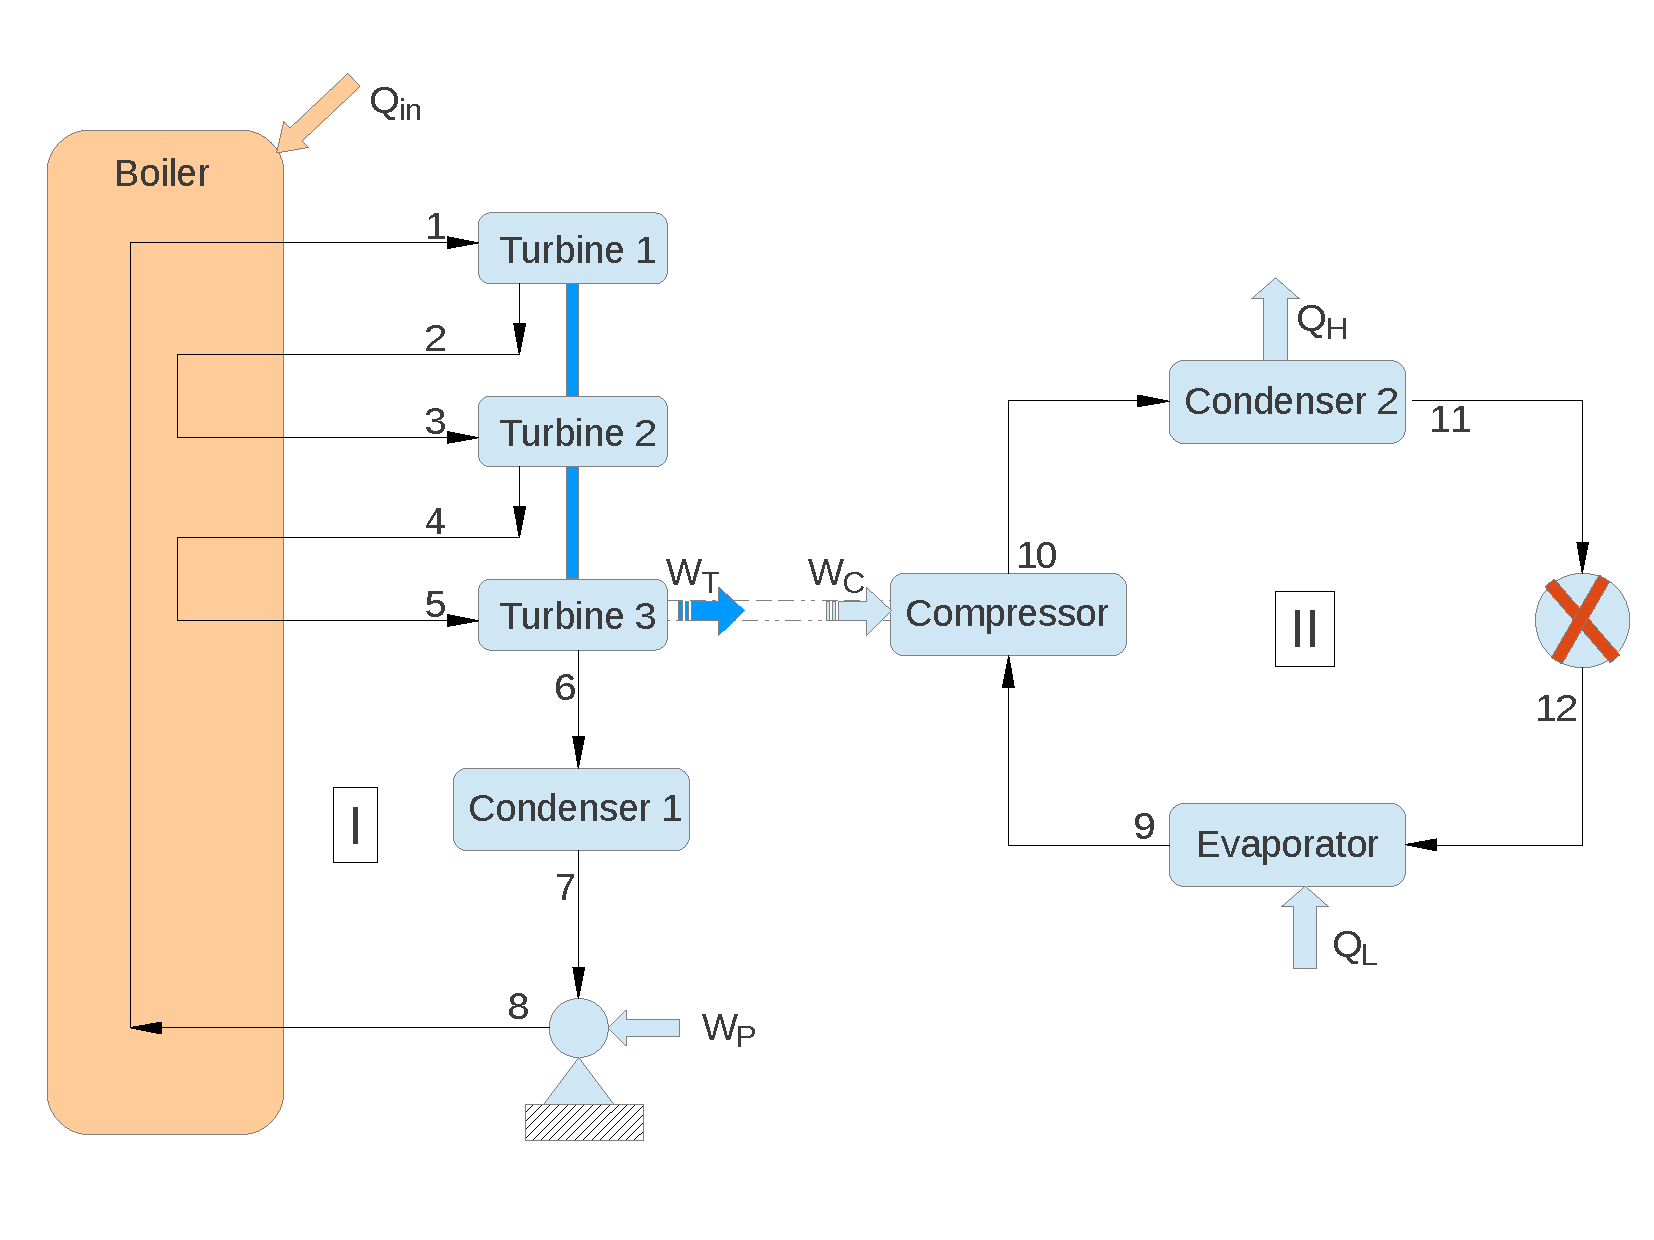
\includegraphics[width=16.0cm,height=12.0cm]{./Pics/Overview_Refrig43}
\end{center}
\caption{Coupled reheat Rankine steam and reversed-Rankine refrigeration units --  Problem \ref{Ex14}.}\label{Ex14:Fig}
\end{figure}

\begin{table}[h]
\begin{center}
\begin{tabular}{ || c || c | c | c | c | c || c ||}
\hline\hline
{\bf Flow}& {\bf Pressure}  &  {\bf Temperature}   &  {\bf Enthalpy}  & {\bf Entropy}     & {\bf State}  & {\bf Quality of} \\
          & {\bf (bar)}     & {\bf ($^{\text{o}}$C)} &  {\bf (kJ/kg)}   &  {\bf (kJ/kg.K)}  &              & {\bf steam}      \\
\hline\hline
{\bf 1}   &   200.0         &      600         &      (A)          &      (B)             & (C)          &  --              \\
{\bf 2}   &   5.0           &       --         &      (D)          &      --              & --           &  (E)             \\
{\bf 3}   &   5.0           &      240         &      (F)          &      (G)             & (H)          &  --              \\
{\bf 4}   &   1.0           &      --          &      (I)          &      --              & --           &  (J)             \\ 
{\bf 5}   &   1.0           &    99.63         &      (K)          &     (L)              &  (M)         &   --             \\ 
{\bf 6}   &   0.23          &      --          &      (N)          &     --               &  --          &  (O)             \\
{\bf 7}   &   (P)           &      --          &      (Q)          &      (R)             &  (S)         &   --             \\              
{\bf 8}   &   (T)           &      --          &      (U)          &       --             & (V)          & --               \\
\hline \hline
{\bf 9}   &   2.0           &      --          &      (i)          &      (ii)            &  (iii)       &  --              \\
{\bf 10}  &  16.0           &     (iv)         &      (v)          &      (vi)            &   (vii)      &   --             \\ 
{\bf 11}  &  (viii)         &     --           &      (ix)         &      --              &  (x)         &   --             \\
{\bf 12}  &   (xi)          &    --            &     (xii)         &      --              &   --         &    --            \\ 
\hline\hline
\end{tabular}
\end{center}
\caption{Information on the steam-power and refrigeration cycles (Problem \ref{Ex14}).}\label{Ex14:Tab1}
\end{table}

\begin{table}[h]
\begin{center}
\begin{tabular}{||c | c c c c | c||}
\hline\hline
               &  {\bf Turbine 1} & {\bf Turbine 2}  & {\bf Turbine 3}  & {\bf Pump}  & {\bf Compressor}\\
{\bf Efficiency}&    0.88          &   0.85           &     0.85         &  0.92      &  1.00           \\
\hline\hline
\end{tabular}
\end{center}
\caption{Efficiencies of the equipment used in the coupled units (Problem \ref{Ex14}).}\label{Ex14:Tab2}
\end{table}


\begin{table}[h]
\begin{center}
\begin{tabular}{|c c| c c c c c c | }
\hline
$P$             & $T_{s}$   & $V_{f}\times 10^{-3}$  &  $V_{g}$   & $H_{f}$  & $H_{g}$   &  $S_{f}$   &  $S_{g}$    \\
(bar)   &  ($^{\text{o}}$C)  & $\left(\text{m}^{3}/\text{kg}\right)$ & $\left(\text{m}^{3}/\text{kg}\right)$ & (kJ/kg) & (kJ/kg) & (kJ/(kg.K)) &  (kJ/(kg.K))  \\
\hline
2.00    &  -18.86  & 1.5071  &  0.5946   &   93.80  & 1419.31  &  0.3843  & 5.5969   \\
16.00   &   41.03  & 1.7306  &  0.0808   &  376.46  &  1470.23 &  1.3729  & 4.8542   \\
\hline
\end{tabular}
\end{center}
\caption{Thermodynamic properties of refrigerant fluid $\mathcal{X}$ (Problem \ref{Ex14}).}\label{Ex14:Tab3}
\end{table}



\end{enumerate}
%\pagebreak
%%%
%\subsection{XXX}
